%\Section 3: Design
%\section{Motivation and Design}
%Section 3: Motivations and Core Challenges
Drawing upon our practical experience integrating AGREE within MBSE workflows, in this section we highlight central challenges and key design principles that guided the development of our LLM-based solution for generating actionable counterexample explanations and facilitating automated model repairs.

\subsection{Context-Aware Prompt Construction}
AGREE-generated counterexamples typically involve numerous variables, intricate execution traces, and extensive AADL architectural data. Incorporating detailed LLM-generated code explanations and diagnostics exacerbates this challenge. Presenting these details directly to a generative AI model without careful management %often exceeds context limitations, resulting in poor or misleading responses. 
often result in excessive context size, increasing latency, hallucinations, costs, and potentially exceeding token limits.
The key challenge is identifying and selecting only the most relevant context to include in prompts, ensuring accurate, concise explanations and actionable recommendations.

\subsection{Ensuring Validity of Automated Repairs}
Generative models might propose repairs that, while plausible, could unintentionally violate established architectural interfaces or critical system properties. Maintaining consistency within compositional reasoning frameworks, such as AGREE, requires continuous validation. Thus, repairs must be tightly integrated with formal verification steps to ensure that each modification preserves overall system correctness.

\subsection{Minimizing User Effort and Interaction Latency}
Manually reviewing detailed logs and deeply nested temporal logic from counterexamples is both error-prone and time-consuming. An effective repair process must significantly reduce user overhead by automating log analysis, semantic comparisons between successive runs, and managing formal proof re-validation. Minimizing both system latency and human interaction time is essential to achieve an efficient, near-interactive model repair workflow.

%%%%%%%%%%%%%%

\begin{figure}[t]
  \centering
  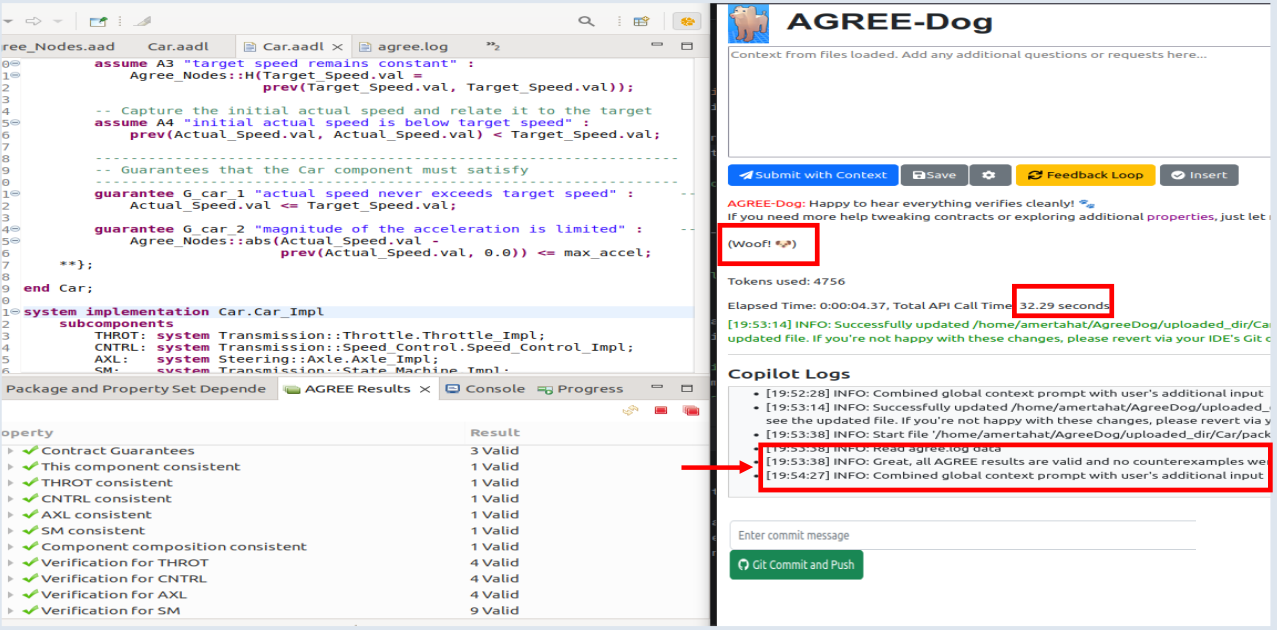
\includegraphics[width=\linewidth]{woof-pic-6.png}
  \caption{AGREE-Dog UI interface showing integrated model diagnostics, user input, token count, response time, and push-button feedback loop. Each repair cycle is proof-aware and synchronized with AGREE log results.}
  \label{fig:copilot-ui}
\end{figure}